\documentclass{article}
    % General document formatting
    \usepackage[margin=0.7in]{geometry}
    \usepackage[parfill]{parskip}
    \usepackage{amsopn}
    \usepackage{mathtools}
    \usepackage[utf8]{inputenc}
    \usepackage{hyperref}
    \usepackage{multicol}
    \usepackage{amsmath,amssymb,amsfonts,amsthm}
    \usepackage{dot2texi}
    \usepackage{tikz}
    \usepackage{mdframed}
    \usetikzlibrary{shapes,arrows}

    \DeclareMathOperator{\StringT}{StringT}
    \DeclareMathOperator{\NumberT}{NumberT}
    \DeclareMathOperator{\BooleanT}{BooleanT}
    \DeclareMathOperator{\LitT}{LitT}
    \DeclareMathOperator{\JSLit}{JSLit}
    \DeclareMathOperator{\JSTypeof}{JSTypeof}
    \DeclareMathOperator{\RecT}{RecT_\Gamma}
    \DeclareMathOperator{\ObjT}{ObjT_\Gamma}
    \DeclareMathOperator{\ListT}{ListT_\Gamma}
    \DeclareMathOperator{\SetT}{SetT_\Gamma}
    \DeclareMathOperator{\MapT}{MapT_\Gamma}
    \DeclareMathOperator{\ObjType}{ObjType}
    \DeclareMathOperator{\UnionT}{UnionT_\Gamma}
    \DeclareMathOperator{\InterT}{InterT_\Gamma}
    \DeclareMathOperator{\LookupObjRef}{\Gamma}
    \DeclareMathOperator{\String}{String}
    \DeclareMathOperator{\Number}{Number}
    \DeclareMathOperator{\Boolean}{Boolean}
    \DeclareMathOperator{\type-ref}{ref}
    \DeclareMathOperator{\Type}{Type_\Gamma}
    \DeclareMathOperator{\NoSuper}{NoSuper}
    \DeclareMathOperator{\InterOrObj}{InterOrObj}
    \DeclareMathOperator{\ObjectSubtype}{ObjectSubtype_\Gamma}
    \DeclareMathOperator{\RecordSubtype}{RecordSubtype}
    \DeclareMathOperator{\Value}{Value_\Sigma}
    \DeclareMathOperator{\StringV}{StringV}
    \DeclareMathOperator{\NumberV}{NumberV}
    \DeclareMathOperator{\BooleanV}{BooleanV}
    \DeclareMathOperator{\RecV}{RecV_\Sigma}
    \DeclareMathOperator{\ObjV}{ObjV_\Sigma}
    \DeclareMathOperator{\ListV}{ListV_\Sigma}
    \DeclareMathOperator{\SetV}{SetV_\Sigma}
    \DeclareMathOperator{\MapV}{MapV_\Sigma}
    \DeclareMathOperator{\UnionV}{UnionV_\Sigma}
    \DeclareMathOperator{\ValueType}{ValueType_\Sigma}
    \DeclareMathOperator{\textref}{ref}
    \DeclareMathOperator{\ObjFields}{ObjFields}
    \DeclareMathOperator{\ObjPairsMatch}{ObjPairsMatch}
    \DeclareMathOperator{\where}{ where }
    \DeclareMathOperator{\textif}{ if }
    \DeclareMathOperator{\suchthat}{s.t.}
    \newcommand{\ValueRef}{\textref}
    \newcommand{\ValueDeref}[1]{\Sigma(#1)}
    \newcommand{\subtype}{<:_\Gamma}
\begin{document}

\title{Sinap's Type System}
\author{Sheyne Anderson}
\maketitle
\section{Intro}

\textbf{TODO:change voice to ``We"}

Sinap IDE is a program to allow editing of graph
programs in various graph programming langauages. Each of these 
languages are loaded into Sinap as ``plugins" and are 
referred to as interpreters. More information 
about the editor can be found at 
\href{https://2graphic.github.io}{2graphic.github.io}.
Because the goal of Sinap IDE is to be an editor for many 
different graph-languages we designed the user interface (UI)
to change to best support the plugin that is currently loaded. 

The idea is that while editing a graph, components of the
graph will have different attributes associated with them 
that the editor should present contextually. For example, in
a graph-language describing deterministic finite-state 
automata (DFAs) edges should have a ``symbol" attribute of 
type character corresponding to the input by which this 
edge should be followed. 

\begin{figure}[h]
    \centering
    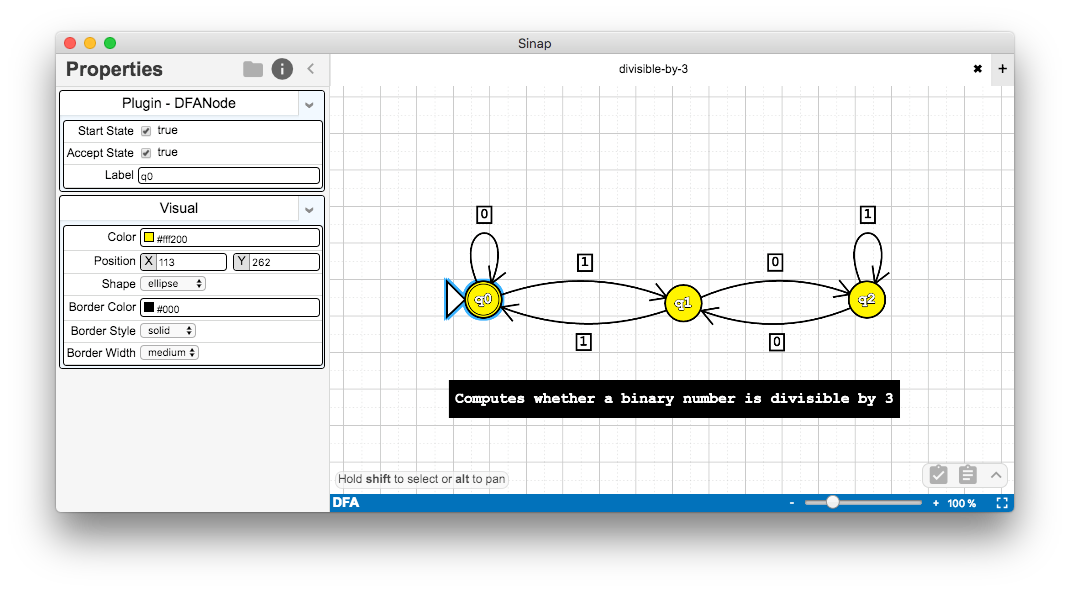
\includegraphics[width=.8\textwidth]{sinap-screenshot}
    \caption{Sinap IDE editing a graph}
    \label{sinap-screenshot}  
\end{figure}

As you can see in Figure \ref{sinap-screenshot}, Sinap's UI
presents the user with nodes and edges which can be selected 
and edited in the sidebar. Allowing the sidebar to change based
on which interpreter is loaded is the purpose of Sinap's Type System. 
This document is presents a model for the type system. 
    
Sinap's Type System consists of two parts:

\begin{enumerate}
    \item A data-language to describe graph components 
    (implemented in values.ts)
    \item A data-description language to define valid schema 
    (implemented in types.ts)
    for the data language
\end{enumerate}

The code for both can be found at 
\href{https://github.com/2graphic/sinap-types}
{github.com/2graphic/sinap-types}.

The data that are allowable in the sidebar can be more complicated than
simple strings and numbers. In the example above the ``Position" attribute
of the node has a structure that similar to the following TypeScript code:

\begin{samepage}
\begin{verbatim}
type Point = {
    x: number;
    y: number;
}
\end{verbatim}
\end{samepage}

Complex types aren't limited to fields directly on nodes and edges,
and can be arbitrarily nested. 

The goal of creating Sinap's Type System is to allow interpreter 
implementers to specify what 
kinds of graphs are valid for their interpreter. This means that 
the interpreter specifies the various fields on nodes and edges 
and can assume that those fields are present on all of the graph elements
that it receives. It also allows different kinds of nodes and edges to
exist in the same graph and allows for rules defining what kinds of
nodes can connect to which edges. 

\section{Types}

\subsection{Notation}

The symbol \((\operatorname{Kind}_1, ...)\) is equivalent to 
\((\operatorname{Kind}_i)\). They are also equivalent to 
\((\operatorname{Kind}_1, ..., \operatorname{Kind}_n)\)
where \(n\) is unspecified and represent an ordered list 
of \(n\) elements. \(\{\operatorname{Kind}_i\}\) represents 
the set of the elements of the list. 

``\(\_\)'' represents a symbol that has been omitted for brevity.

\subsection{Type Model}
The data-description language is called Sinap Types. There are 
several kinds of types:

\begin{itemize}
    \item \(\LitT(\JSLit)\) is the type for literal primitives. That is
    string, number, and boolean literals. 
    Examples include \(\LitT(17), \LitT(\text{``Hello"}), \text{ and } 
    \LitT(false)\). A value will match this type if and only if it is
    exactly the value of the literal in the type. 
    \item \(\StringT\) is a type matching all strings.
    \item \(\NumberT\) is a type matching all numbers.
    \item \(\BooleanT\) is a type matching all booleans.
    \item \(\RecT((\String, \Type)...)\) is a type for records. 
    The arguments come in pairs of \((\String, \Type)\) where
    \(\String\) is the name of some field and \(\Type\) is the
    type of that field.
    \item \(\ListT(\Type)\) is a type for homogeneous lists. The
    parameter is the type of all the elements of the list. 
    \item \(\SetT(\Type)\) is a type for an unordered collection
    of elements of type \(\Type\).
    \item \(\MapT(\Type_1, \Type_2)\) is the type of a mapping from 
    \(\Type_1\) to \(\Type_2\).
    \item \(\ObjT(\String, \String | \NoSuper, ((\String, \Type), ...))\)
    describes an object type. Its name is the first argument, 
    its super-type is the second argument, and the new fields 
    it introduces is the tuple of (key, value) pairs that form the
    last argument. 
    \item \(\InterT(\ObjT,  ...)\) is the intersection of several 
    object types and acts like a single object type with all the 
    properties of the intersected types. 
    \item \(\UnionT(\Type, ...)\) is a union of several types. 
    Values with this type act as a collection with a single element
    whose type is one of the \(\{\Type_i\}\). In Sinap, a drop down 
    menu that allows ``Narrow'', ``Wide'', or some number would be 
    typed as \(\UnionT(\LitT(``\text{Narrow}"), \LitT(``\text{Wide}"),
     \NumberT)\).
\end{itemize}

These informal descriptions of the various types is recognized formally 
in Figure \ref{sinap-types-model}.

\begin{figure}
\begin{mdframed}
\begin{align*}
\begin{aligned}
\Type = &\LitT(\JSLit) \\
&|\StringT \\
&|\NumberT \\
&|\BooleanT \\
&|\RecT((\String, \Type), ...) \\
&|\ListT(\Type) \\
&|\SetT(\Type) \\
&|\MapT(\Type, \Type) \\
&|\ObjT\left(\begin{aligned}
    &\String, \String | \NoSuper, \\
&((\String, \Type), ...)
\end{aligned}\right) \\
&|\InterT(\ObjT, ...) \\
&|\UnionT(\Type, ...)\\
\end{aligned}
\quad\quad\quad\begin{aligned}        
\begin{aligned}
\JSLit = &\operatorname{JSString} \\
&| \operatorname{JSNumber} \\
&| \operatorname{true} \\
&| \operatorname{false} \\
\end{aligned}\\\\
\begin{aligned}
\JSTypeof(\operatorname{JSString}) &= \StringT \\
\JSTypeof(\operatorname{JSNumber}) &= \NumberT \\
\JSTypeof(\operatorname{true}) &= \BooleanT \\
\JSTypeof(\operatorname{false}) &= \BooleanT \\
\end{aligned}  
\end{aligned}  
\end{align*}
\end{mdframed}
\caption{Formal Description of Sinap Types}
\label{sinap-types-model}
\end{figure}

\subsection{Subtype Relations}

With types defined, it is necessary to define a subtype 
relation (\(\bullet\subtype\bullet\)). Subtypes correspond 
roughly to the idea that if \(A\subtype B\) then \(A\)
can be used where \(B\) can be used. 

\begin{figure}
\begin{mdframed}        
\begin{align*}
    \Type_1&\subtype\Type_1 \\
    \LitT(\JSLit_1)&\subtype\Type_1 &&\textif \JSTypeof(\JSLit_1) = \Type_1 \\
    \InterT(\Type_{1,1}, ...)&\subtype\InterT(\Type_{2,1}, ...) 
    &&\textif \forall T\in \{\Type_{2,i}\} \exists T' \in \{\Type_{1,i}\} \suchthat T'\subtype T \\
    \InterT(..., \Type_i, ...)&\subtype\ObjT_1 &&\textif \ObjT_1 = \Type_i  \\
    \ObjT_1 &\subtype \ObjT(\String_1, \_, \_) &&\textif \ObjectSubtype(\String_1, \ObjT_1)\\
    \RecT_1&\subtype\RecT_2 &&\textif \RecordSubtype(\RecT_1, \RecT_2) \\
    \ListT(\Type_1)&\subtype\ListT(\Type_2) &&\textif \Type_1\subtype\Type_2 \\
    \SetT(\Type_1)&\subtype\SetT(\Type_2) &&\textif \Type_1\subtype\Type_2 \\
    \MapT(\Type_{11}, \Type_{12})&\subtype\MapT(\Type_{21}, \Type_{22}) &&\textif \Type_{11}\subtype\Type_{21} \text{ and } \Type_{12}\subtype\Type_{22} \\
\end{align*}
\begin{align*}
    \ObjectSubtype(\String_1, \ObjT(\String_2,\_, \_)) \quad &\textif 
    \quad (\String_1 = \String_2)\\
    \ObjectSubtype(\String_1, \ObjT(\_,\String_2, \_)) \quad &\textif 
    \quad \ObjectSubtype(\String_1, \LookupObjRef(\String_2)))
\end{align*}
\begin{align*}
    \RecordSubtype &\left(\begin{aligned}
        &\RecT((\String_{1,1}, \Type_{1, 1}), ..., (\String_{1,n}, \Type_{1, n})), \\
        &\RecT((\String_{2,1}, \Type_{2, 1}), ..., (\String_{2,m}, \Type_{2, m}))
    \end{aligned}\right) \\
    &\textif \{\String_{2,i}\} \subset \{\String_{1,i}\} \text{ and } \String_{1, i} = \String_{2, j} \implies \Type_{1, i} \subtype \Type_{2, j}
\end{align*}
\end{mdframed}        
    \caption{Rules for the subtype relation (\(\bullet\subtype\bullet\))}
\label{subtype-definitions}
\end{figure}

Note that this actually allows for some weirdness, because 
we lose some of the restrictions of the subtype Map when using
it as the supertype. This is incredibly unlikely in the use case 
of Sinap because data aren't reused between different nodes and
edges. 

Records are structurally typed, two records with the same structure have
the same type. Objects are nominally typed, so the type system needs some
notion of references to support them. 

While Sinap's Type System is implemented as a library and can have 
concrete syntaxes in several languages, our most mature implementation 
is in TypeScript. 

An example of how this translation is applied is given in Figure \ref{types-example}. 

\begin{figure}
\begin{mdframed}
\begin{align*}
    \text{Nodes} = &\UnionT\left(
        \begin{aligned}
        &\ObjT\left(
            \begin{aligned}    
                \text{``Node1"}, \NoSuper, \left(
                    \begin{aligned}
                        &(\text{``label"}, \StringT),  \\
                        &(\text{``customAttribute"}, \NumberT)
                    \end{aligned}\right)
            \end{aligned}\right),  \\
        &\ObjT\left(\text{``Node2"}, \NoSuper, \left(\begin{aligned}
            (&\text{``label"}, \StringT),  \\
            (&\text{``otherAttribute"}, \RecT\left(
                \begin{aligned}
                    (&\text{``f1"}, \BooleanT),  \\
                    (&\text{``f2"}, \NumberT)
                \end{aligned}\right)
        \end{aligned}\right)\right)
        \end{aligned}\right)  \\
    \text{Edges} = &\UnionT\left(\ObjT\left(
        \text{``Edge"}, \NoSuper,  
        \left(\begin{aligned}
            (&\text{``label"}, \StringT), \\
            (&\text{``source"}, \ObjT(\text{``Node1"}, \_, \_)), \\
            (&\text{``destination"}, \ObjT(\text{``Node2"}, \_, \_)) \\             
        \end{aligned}\right)\right)\right)
\end{align*}
\end{mdframed}
\caption{An example of an interpreter's description of valid graphs}
\label{types-example}
\end{figure}
The types described in Figure \ref{types-example} are
can be written in TypeScript as shown in Figure \ref{types-example-code}.

\begin{figure}
\begin{mdframed}    
\begin{verbatim}
class Node1 {
    label: string;
    customAttribute: number;
}

class Node2 {
    label: string;
    otherAttribute: {
        f1: boolean,
        f2: number
    };
}

class Edge {
    label: string
    source: Node1;
    destination: Node2;
}

type Nodes = Node1 | Node2;
type Edges = Edge;
\end{verbatim}
\end{mdframed}
\caption{TypeScript code to go with Figure \ref{types-example}}
\label{types-example-code}
\end{figure}

\section{Values}

Now that we have a description of valid graph structures for some
interpreter, we need to define a language for describing specific 
graphs. 

Note that Values are parameterized by \(\Sigma\), a ``store" that
allows Values to reference other values without including their 
whole structure. This allows for cycles. 

\textbf{TODO: specifically \(\Sigma\) maps refs to values}

\begin{align*}
    \Value =& \StringV(\Type_1, \String_1) \quad\where \Type_1 \subtype \StringT \\
    &| \NumberV(\Type_1, \Number_1) \quad\where \Type_1 \subtype \NumberT \\
    &| \BooleanV(\Type_1, \Boolean_1) \quad\where \Type_1 \subtype \BooleanT \\
    &| \ObjV(\Type_1, V=((\String_1, \ValueRef_1]), ...)) \quad\where 
    \ObjPairsMatch(\ObjFields(\Type_1), V) \\
    &| \UnionV(\UnionT(..., \Type_i, ...), \ValueRef_1) \where
    \ValueType(\ValueRef_1) \subtype \Type_i\\
    &| \ListV(\ListT(\Type_1), (\ValueRef_1, ...)) \where \ValueType(\ValueRef_i) \subtype \Type_1 \\
    &| \SetV(\SetT(\Type_1), \{\ValueRef_1, ...\}) \where \ValueType(\ValueRef_i) \subtype \Type_1 \\
    &| \MapV(\MapT(\Type_1, \Type_2), ((\ValueRef_{1,1}, \ValueRef_{2,1}), ...)) \where \bigwedge
    \begin{aligned}
        \ValueType(\ValueRef_{1, i}) \subtype \Type_1 \\
        \ValueType(\ValueRef_{2, i}) \subtype \Type_2 
    \end{aligned}\\
\end{align*}

\begin{align*}
    \ObjFields(\ObjT(\_, \String_S, (P_1 = (\String_1, \Type_1), ...))) &= \operatorname{concat}(\ObjFields(\LookupObjRef(\String_S), (P_n))) \\
    \ObjFields(\InterT(ObjT_1, ...)) &= \operatorname{concat}(\ObjFields(\ObjT_1), ...)
\end{align*}

\begin{align*}
    \ValueType(\ValueRef_1) &= \ValueType(\ValueDeref{\ValueRef_1}) \\
    \ValueType(\StringV(\Type_1, \_)) &= \Type_1 \\
    \ValueType(\NumberV(\Type_1, \_)) &= \Type_1 \\
    \ValueType(\BooleanV(\Type_1, \_)) &= \Type_1 \\
    \ValueType(\ObjV(\Type_1, \_)) &= \Type_1 \\
    \ValueType(\UnionV(\Type_1, \_)) &= \Type_1 \\
    \ValueType(\ListV(\Type_1, \_)) &= \Type_1 \\
    \ValueType(\SetV(\Type_1, \_)) &= \Type_1 \\
    \ValueType(\MapV(\Type_1, \_)) &= \Type_1 \\
\end{align*}
\begin{align*}
    \ObjPairsMatch(((\String_1, \Type_1),...), ((\String_1, \ValueRef_1), ...)) 
    \textif \forall i, \ValueType(\Value_i) \subtype \Type_i
\end{align*}

A valid graph then matches 
\[(\ListV(\ListT(\textit{Nodes}), \_), \ListV(\ListT(\textit{Edges}), \_))\]
for some appropriate definition of \textit{Nodes} and \textit{Edges}.

\subsection{Example}
\begin{figure}[h]
    \centering
    \begin{dot2tex}[dot, scale=0.5]
    digraph {
        "Start Node" -> "End Node";
    }
    \end{dot2tex}
    \caption{A simple graph}
    \label{simplegraph}
\end{figure}   
To give an example, the simple graph given in Figure \ref{simplegraph} 
might be modeled as:

\newcommand{\treeDraw}[2]{#1 \left(\begin{aligned} &#2\end{aligned}\right)}
\newcommand{\treeNext}{,\\&}
\newcommand{\valRef}[1]{\ValueRef_\textit{#1}}
\newcommand{\textq}[1]{\text{``#1"}}

\begin{align*}
    \Sigma(\valRef{0O})&=\ObjV(\ObjT_0, ())\\ 
    \Sigma(\valRef{0U})&=\UnionV(\UnionT_0, \valRef{0O})\\
    \Sigma(\valRef{1S})&=\treeDraw\StringV{\StringT_1, \textq{Start Node}}\\
    \Sigma(\valRef{1O})&=\treeDraw\ObjV{\ObjT_1,\treeDraw{}{
        (\textq{label}, \valRef{1S})\treeNext
        (\textq{destination}, \valRef{3U})
        }}\\
    \Sigma(\valRef{1U})&=\treeDraw\UnionV{\UnionT_1, \valRef{1O}}\\
    \Sigma(\valRef{2S})&=\treeDraw\StringV{\StringT_2, \textq{End Node}}\\
    \Sigma(\valRef{2O})&=\treeDraw\ObjV{\ObjT_2,\treeDraw{}{
        (\textq{label}, \valRef{2S})\treeNext
        (\textq{destination}, \text{nil})
        }}\\
    \Sigma(\valRef{2U})&=\treeDraw\UnionV{\UnionT_2, \valRef{2O}}\\
    \Sigma(\valRef{3O})&=\treeDraw\ObjV{\ObjT_3,\treeDraw{}{
        (\textq{children}, \valRef{4})
        }}\\
    \Sigma(\valRef{3U})&=\treeDraw\UnionV{\UnionT_3, \valRef{3O}}\\
    \Sigma(\valRef{4})&=\treeDraw\ListV{\ListT_4, (\valRef{2U})}\\
    \textit{Nodes}_1 &= \treeDraw\ListV{\ListT_5, (\valRef{1U}, \valRef{2U})} \\
    \textit{Edges}_1 &= \treeDraw\ListV{\ListT_6, (\valRef{3U})} \\
\end{align*}


\(\Sigma\) can probably better be understood Figure \ref{values-example}.

\begin{figure}[h]
    \centering
    \begin{dot2tex}[fdp, scale=0.5]
    digraph {
        "1U" [label="UnionV (1U)"];
        "2U" [label="UnionV (2U)"];
        "3U" [label="UnionV (3U)"];
        "1O" [label="ObjV (1O)"];
        "2O" [label="ObjV (2O)"];
        "3O" [label="ObjV (3O)"];
        "1S" [label="StringV (1S)"];
        "2S" [label="StringV (2S)"];
        "3S" [label="StringV (3S)"];
        "4" [label="ListV (4)"];
        "1U" -> "1O";
        "1O" -> "1S" [label="label"];
        "2U" -> "2O" [label="label"];
        "2O" -> "2S";
        "3U" -> "3O";
        "3O" -> "3S";
        "1O" -> "3U" [label="destination"];
        "2O" -> "0U" [label="destination"];
        "3O" -> "4" [label="children"];
        "4" -> "2U"
    }
    \end{dot2tex}
\caption{A diagram of the example Values}
\label{values-example}
\end{figure}

\section{Conclusion}
Sinap types is useful for generically describing data-structures 
so that GUIs for their entry can be automatically generated. 

\textbf{TODO: what do I even say here?}

\textbf{TODO:Things that are not covered}

\textbf{TODO:Discuss the python implementation}
\textbf{TODO:Typescript}

\textbf{TODO:Source/Destination, how is the model actually used?}
\end{document}
